\documentclass[12pt, twoside, a4paper]{report}
\usepackage{amsmath}
\usepackage{ragged2e}
\usepackage{fancyhdr}
\usepackage{graphicx}
\usepackage{float}
\usepackage{hyperref}

\title{CS2810 - Group Report}
\author{Marcus Messer, Toby Such, Roger Milroy, Andrew Nicolalde,\\
Jonathan Lewin, Robin Chabouk, Johan Rehman}
\date{\today}

\begin{document}
\maketitle
\pagestyle{fancy}
\fancyhf{}
\lhead{CS2810 - Group Report}
\rfoot{Page \thepage}

\chapter*{Description Of Components}
\section*{Views}
See \textit{\nameref{sec:static}} for links to the Java Script Documentation.
\subsection*{Customer}
\subsubsection*{Start Order Page}
The Customer Start Order page is the initial page the customer sees.
It contains a carousel element, a Start Order button, and three images. The central Start Order button directs the customer to the menu page. 

See \textit{Figure \ref{fig:startOrder}}

\begin{figure}[H]
  \centering
  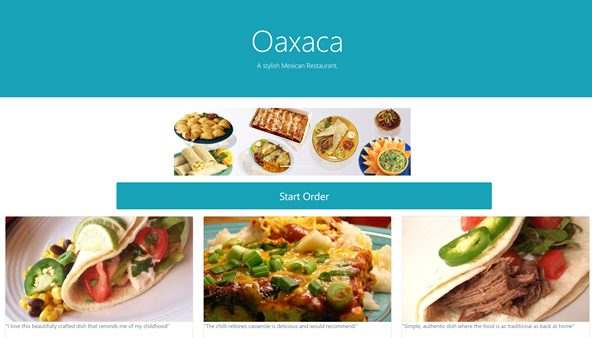
\includegraphics[width=10cm]{startOrder.png}
  \caption{The customer landing page}
  \label{fig:startOrder}
\end{figure}

\subsubsection*{Menu Page}
Once the customer has clicked Start Order, they will be brought to the Menu Page.

The customer can now pick which items they want to order by searching through four different categories.

See \textit{Figure \ref{fig:menuClosed}} and \textit{Figure \ref{fig:menuOpen}}

\begin{figure}[H]
  \centering
  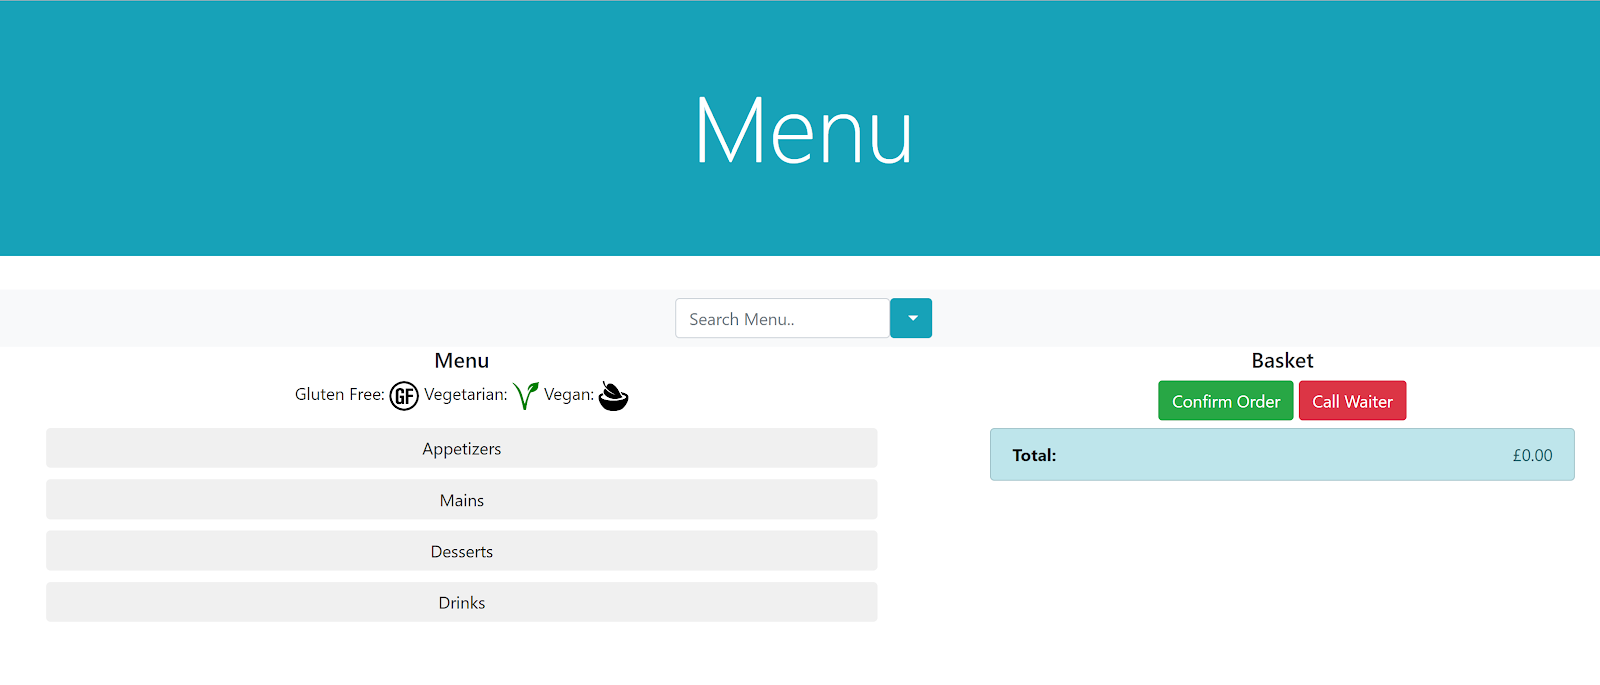
\includegraphics[width=10cm]{MenuClosed.png}
  \caption{The Menu Page with Closed Categories}
  \label{fig:menuClosed}
\end{figure}

\begin{figure}[H]
  \centering
  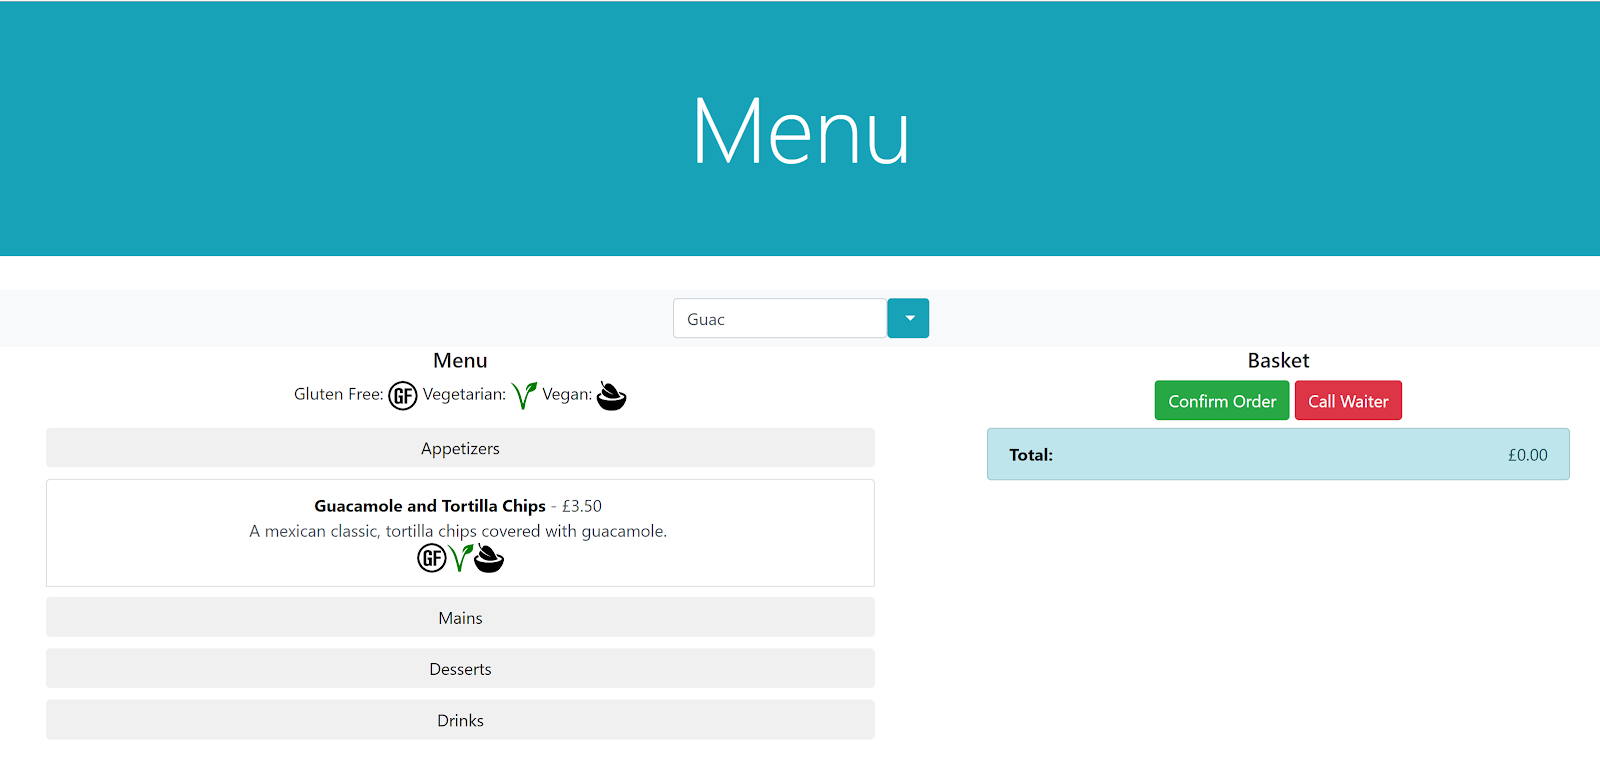
\includegraphics[width=10cm]{MenuOpen.png}
  \caption{The Menu Page with Open Categories}
  \label{fig:menuOpen}
\end{figure}

A customer can also search for an item, filtering by a specific category (vegan/vegetarian/gluten free) which will only display items that meet the category criteria. 

See \textit{Figure \ref{fig:menuFilter}}

\begin{figure}[H]
  \centering
  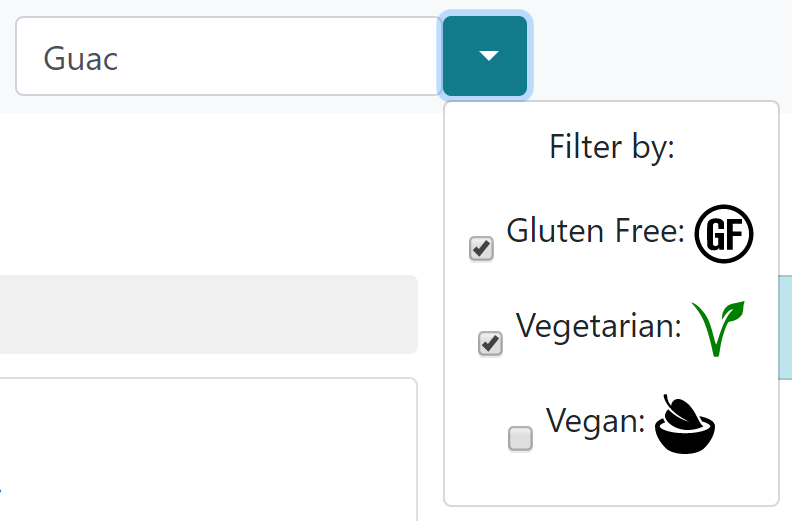
\includegraphics[width=5cm]{MenuFilter.png}
  \caption{The Menu Filtering Section}
  \label{fig:menuFilter}
\end{figure}

Once the customer clicks on the menu item they want to order, an item summary will pop up and will display more information such as the Price and the description of the item.
They can also add specific instructions that will then be seen by the chefs that cook the meal.
When the customer clicks the ‘Add to Order’ button, the order is added to the list.

See \textit{Figure \ref{fig:menuItem}}

\begin{figure}[H]
  \centering
  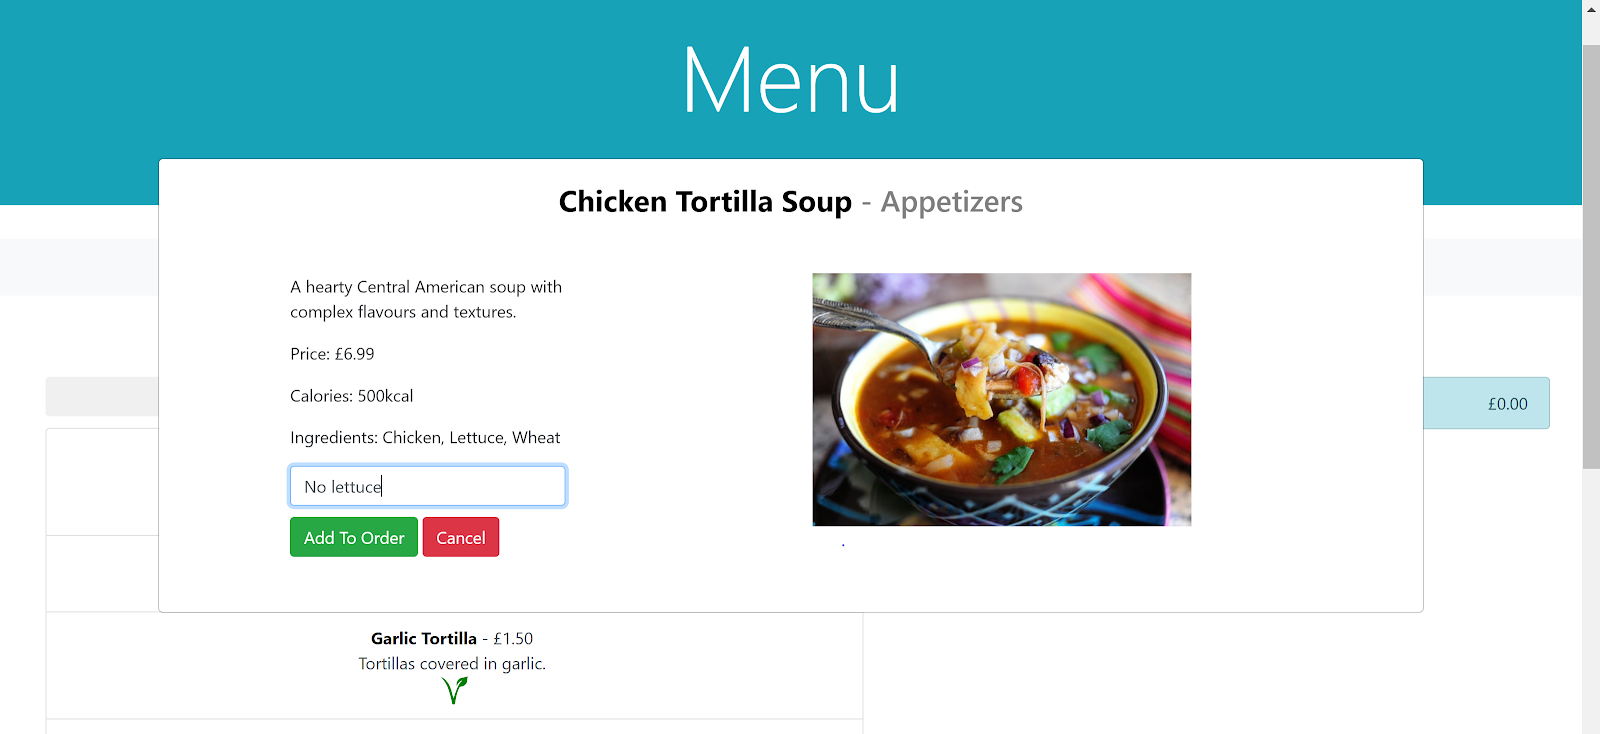
\includegraphics[width=10cm]{MenuItem.png}
  \caption{The Menu Item Modal}
  \label{fig:menuItem}
\end{figure}

The menu items that the customer has added to the order is then displayed under the basket order list.
This list will show the items that have been added, their individual price and the total price.

Once the customer is happy that they have all the items they want to order, they will click ‘Confirm Order’ to send the list to the basket page. 

See \textit{Figure \ref{fig:menuOrder}}

\begin{figure}[H]
  \centering
  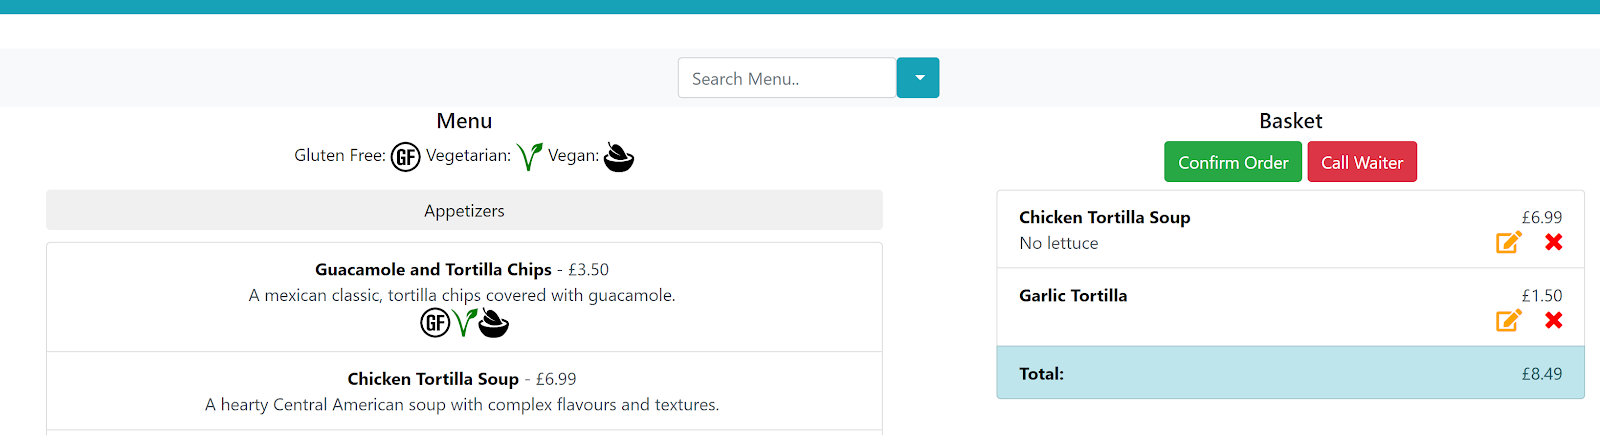
\includegraphics[width=10cm]{MenuOrder.png}
  \caption{The Menu Page with an Order}
  \label{fig:menuOrder}
\end{figure}

\subsubsection*{Basket Page} 

This is the page the customer is taken to once they have selected and confirmed what they want to order.
Customers can add to the same order by navigating to the basket page via the link in the top right of the page, or can start a new order by navigating to the home page.

Each order has an order number, shows the status of the order (along with a little symbol that reflects this) and the price for that order.
Orders contain a table with all the items in that order.
The table includes the name of each item, a short description, any instructions that were added and the price.
If more than one of the same item is added to the order, it is shown by a repetition of the item in the order table.

At the bottom of the accordion element the total price is displayed for all orders so that customers have an up to date idea of how much their meal is costing them.
The call waiter button simply notifies a waiter that the particular table needs assistance and confirms with the customer that this has been done via a modal.
There is also a back to menu button next to call waiter for convenience.

This view gives the customer a good idea of what is going on with their orders and allows them to plan what else they may want to get accordingly.

See \textit{Figure \ref{fig:basket}}

\begin{figure}[H]
  \centering
  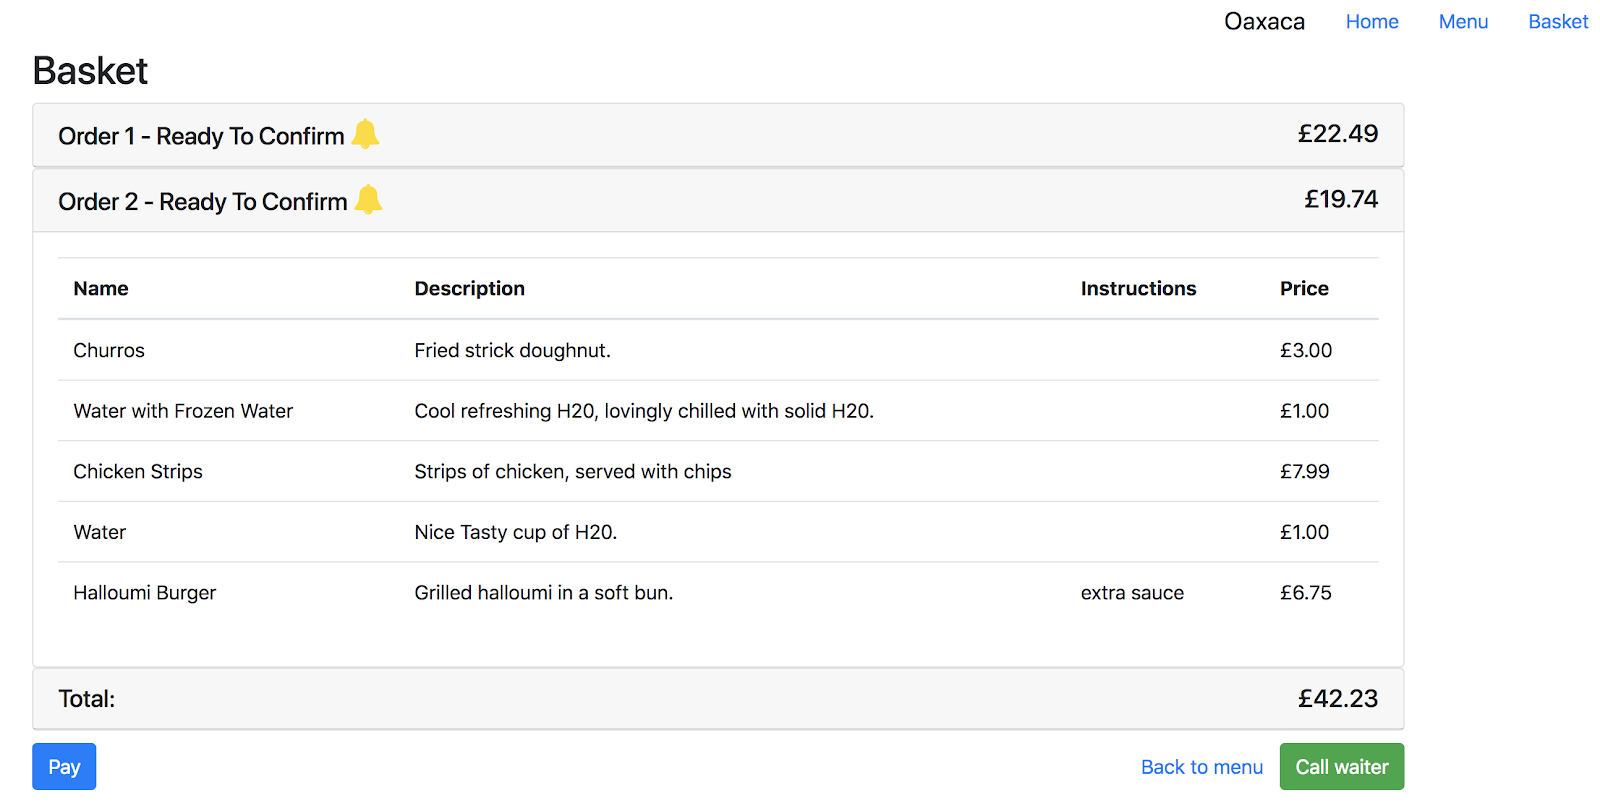
\includegraphics[width=10cm]{basket.png}
  \caption{The Customer's Basket Page}
  \label{fig:basket}
\end{figure}

\subsubsection*{Payment}
This is the payment form, see \textit{Figure \ref{fig:pay}}. It forms a part of the Basket page and is made visible when the pay button is pressed.

On this page, the customer enters several details. Their email address is used to send the customer an email receipt, and their card details are used to debit their account.
The user enters these details and then clicks the “Pay” button, which also displays the total for the Transaction.
Upon successful payment, the customer will be redirected to the start order page and they will be free to leave.

\begin{figure}[H]
  \centering
  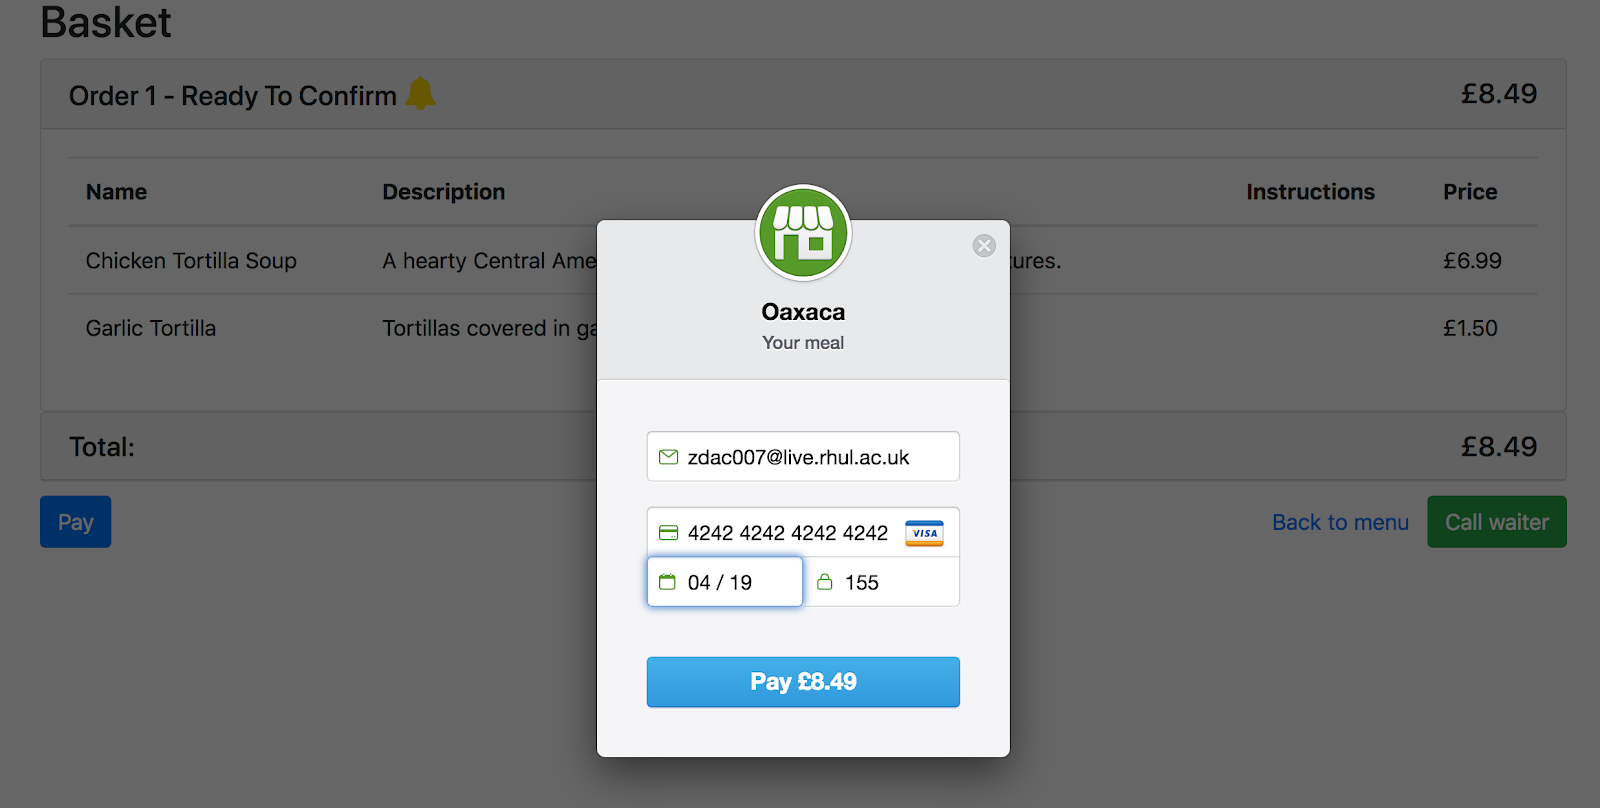
\includegraphics[width=10cm]{Payment.png}
  \caption{The Customer's Payment Form}
  \label{fig:pay}
\end{figure}

\subsection*{Waiter}
\subsubsection*{Orders Page}
This is the view the waiter sees, on the left is the list of tables that the waiter is assigned to.
On the right is the details of the order that the waiter has selected.
There are a number of symbols to show the waiter at a glance the state of their tables once they have learnt them.
There are action buttons that modify the state of the selected order and they are activated and deactivated depending on the state of the order to minimise human error.

See \textit{Figure \ref{fig:orders1}}

\begin{figure}[H]
  \centering
  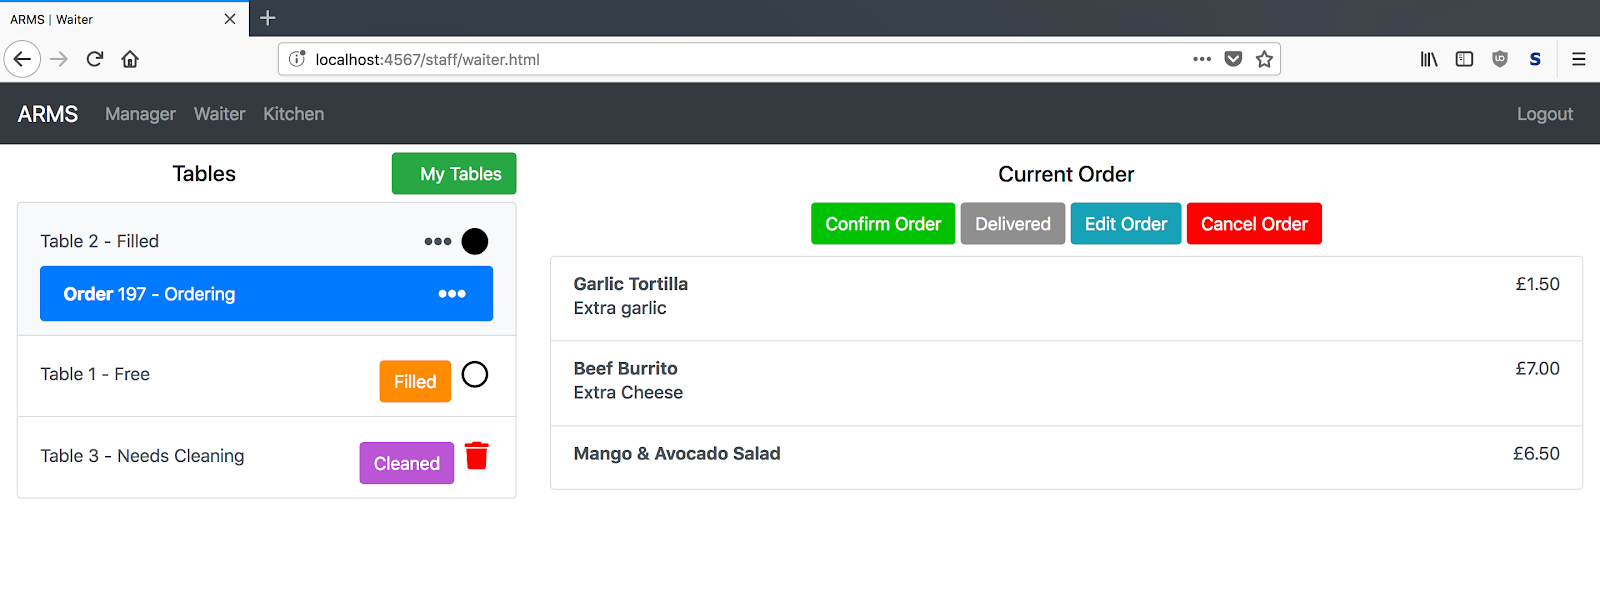
\includegraphics[width=10cm]{orders1.png}
  \caption{Order Page - My Tables}
  \label{fig:orders1}
\end{figure}

The waiter can also press the toggle at the top of the list of tables to see all the tables in the restaurant in case they have to cover another waiters tables for example.

See \textit{Figure \ref{fig:orders2}}

\begin{figure}[H]
  \centering
  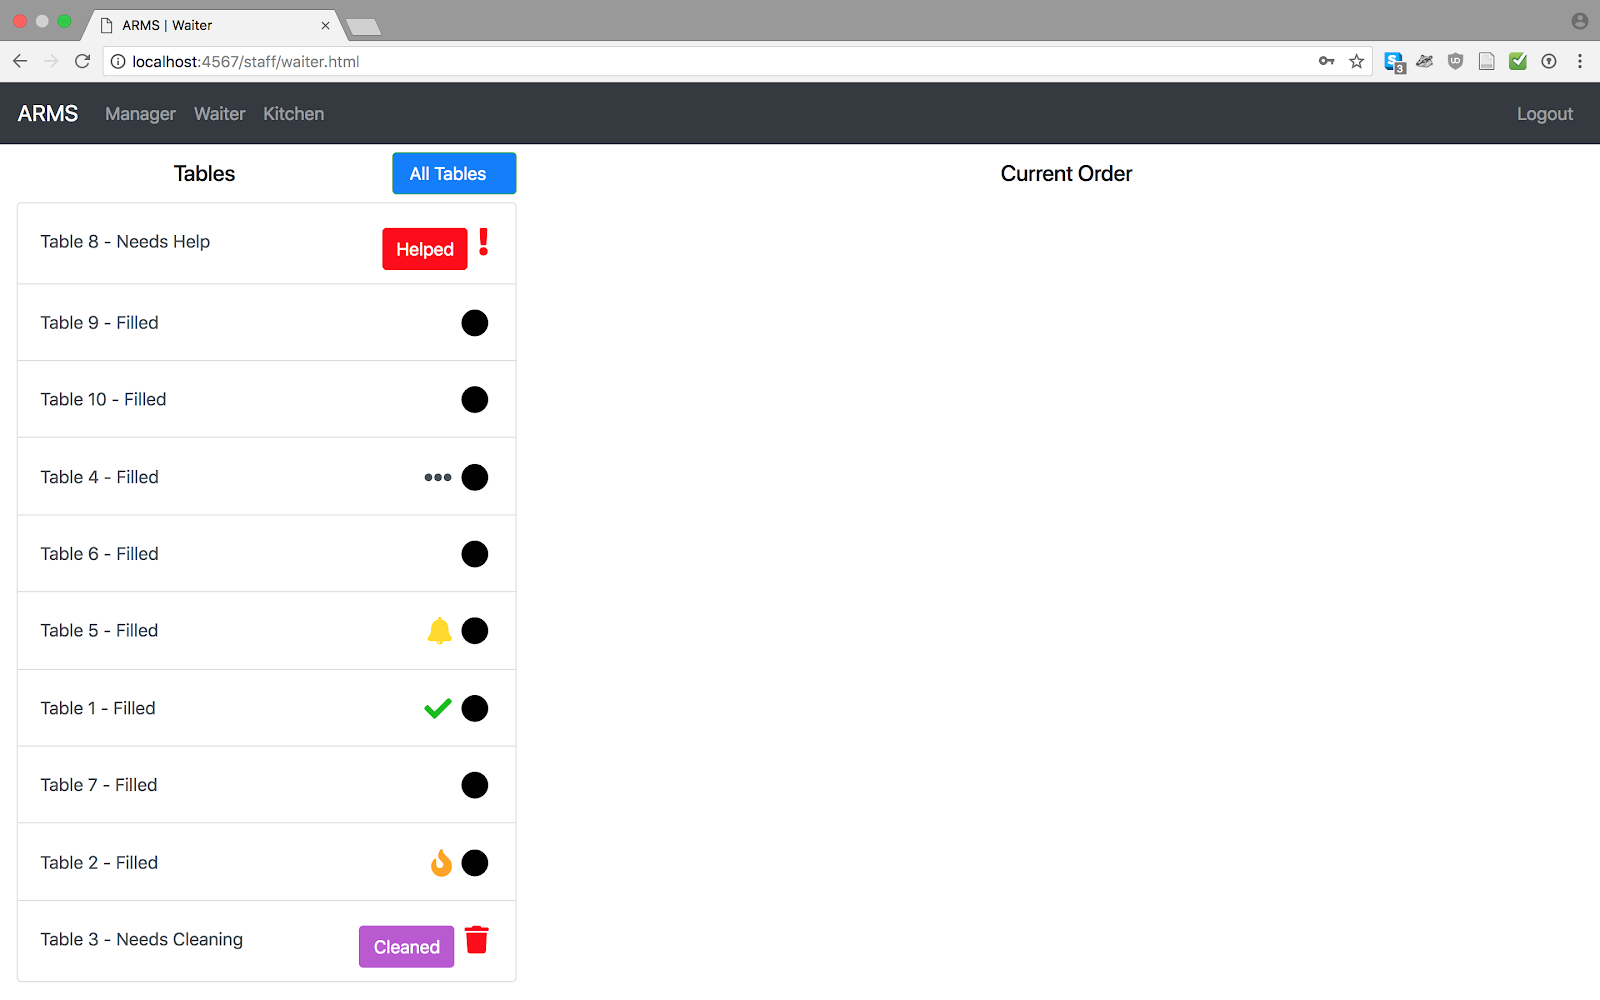
\includegraphics[width=10cm]{orders2.png}
  \caption{Order Page - All Tables}
  \label{fig:orders2}
\end{figure}

When a customer indicates that they are ready to confirm their order a notification appears on the relevant waiters page. This also triggers an update so the most up to date information is displayed.

See \textit{Figure \ref{fig:orders3}}

\begin{figure}[H]
  \centering
  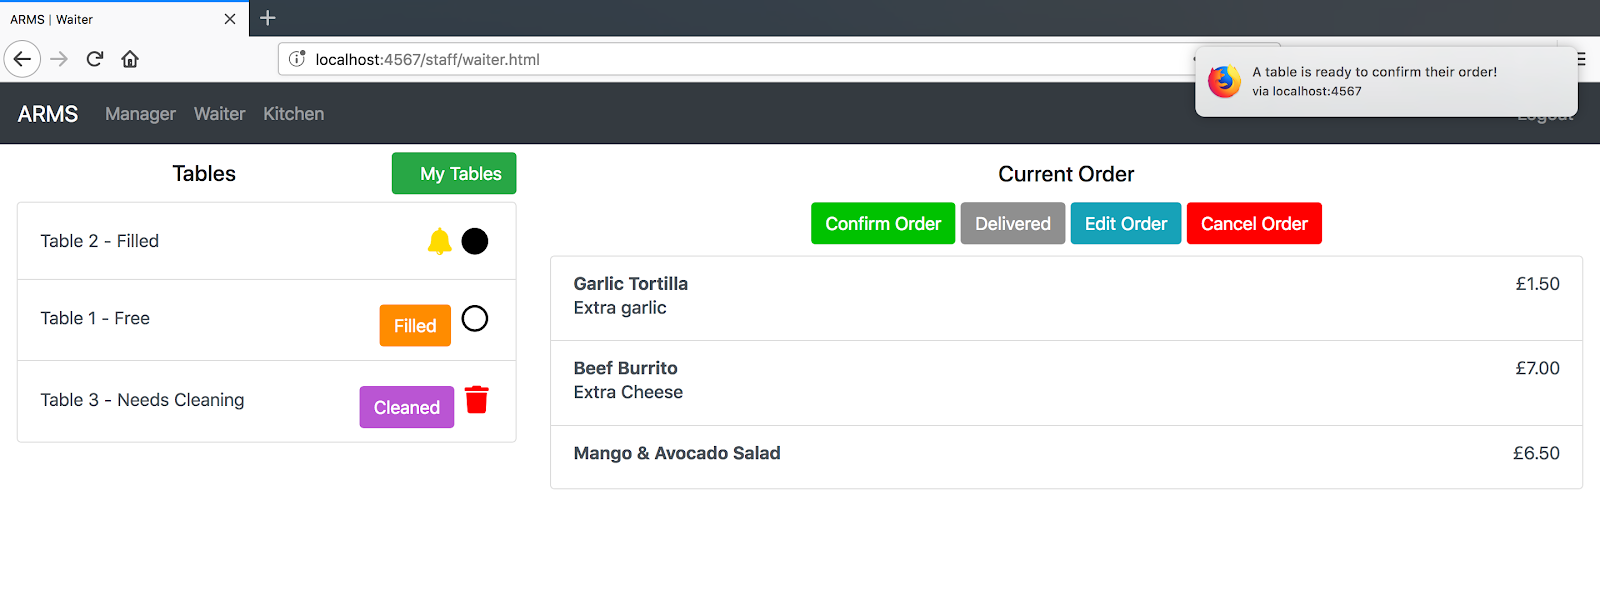
\includegraphics[width=10cm]{orders3.png}
  \caption{Order Page - Selected Order}
  \label{fig:orders3}
\end{figure}

If at any point the customer needs help they can press a button and the waiter will get a notification and the table status indicator will change. This gives a quick visual indicator that action is required.

See \textit{Figure \ref{fig:order4}}

\begin{figure}[H]
  \centering
  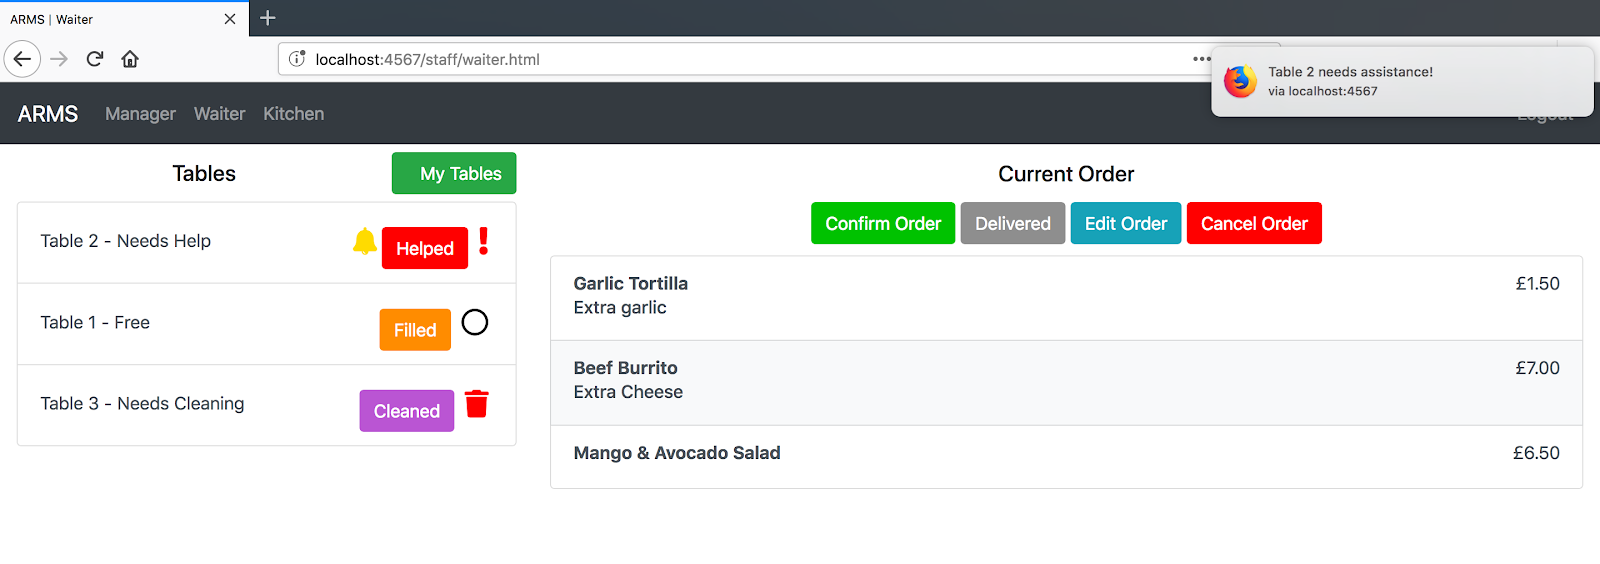
\includegraphics[width=10cm]{orders4.png}
  \caption{Order Page - Notification}
  \label{fig:orders4}
\end{figure}

\subsubsection*{Edit Order View}
This modal allows the waiter to edit a customers order. It loads the customers current order and the menu so that the waiter can add items to the order.

See \textit{Figure \ref{fig:editOrder}}

\begin{figure}[H]
  \centering
  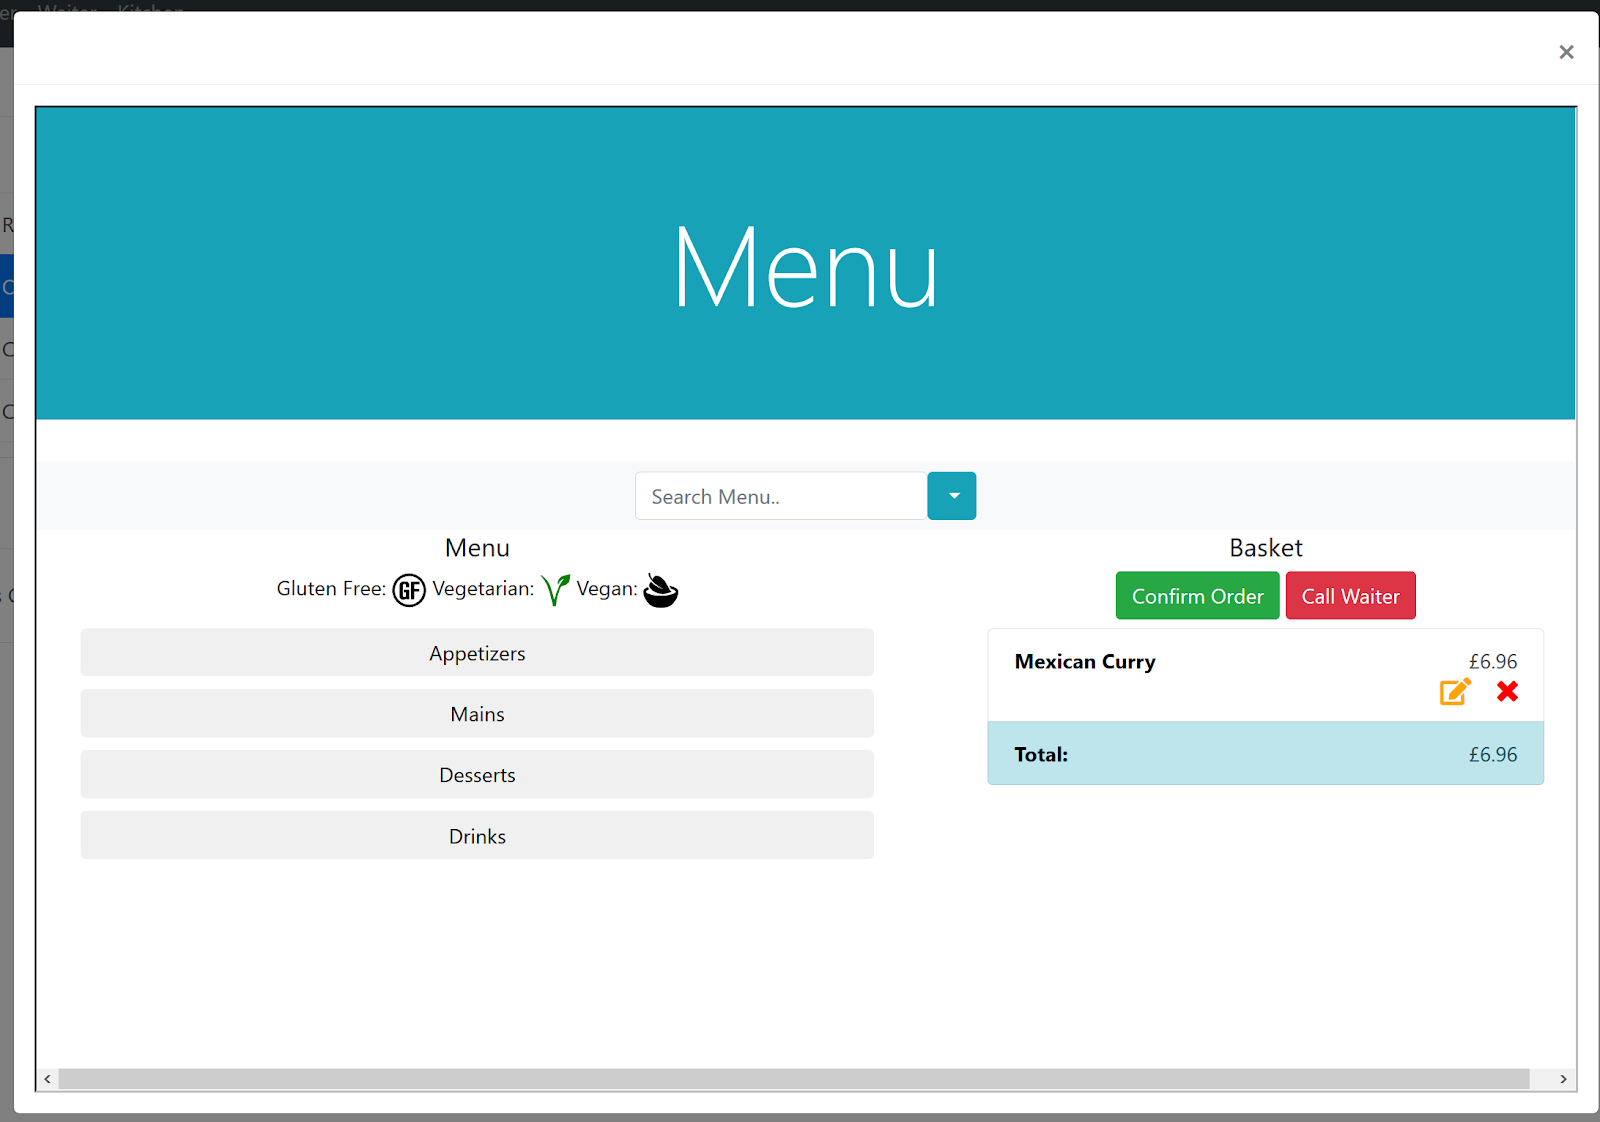
\includegraphics[width=10cm]{editOrder.png}
  \caption{Edit Order}
  \label{fig:editOrder}
\end{figure}

\subsection*{Kitchen}
This is the view the kitchen staff see.
The orders are displayed with the oldest (and most important) in the main part of the page, the background colours are visual cues for the kitchen staff to quickly assess the backlog.
If there are more than 4 orders the list overflows to the sidebar still with background colour indicating priority.
As older Orders are finished they pop off the sidebar onto the main page.

See \textit{Figure \ref{fig:kitchen1}}

\begin{figure}[H]
  \centering
  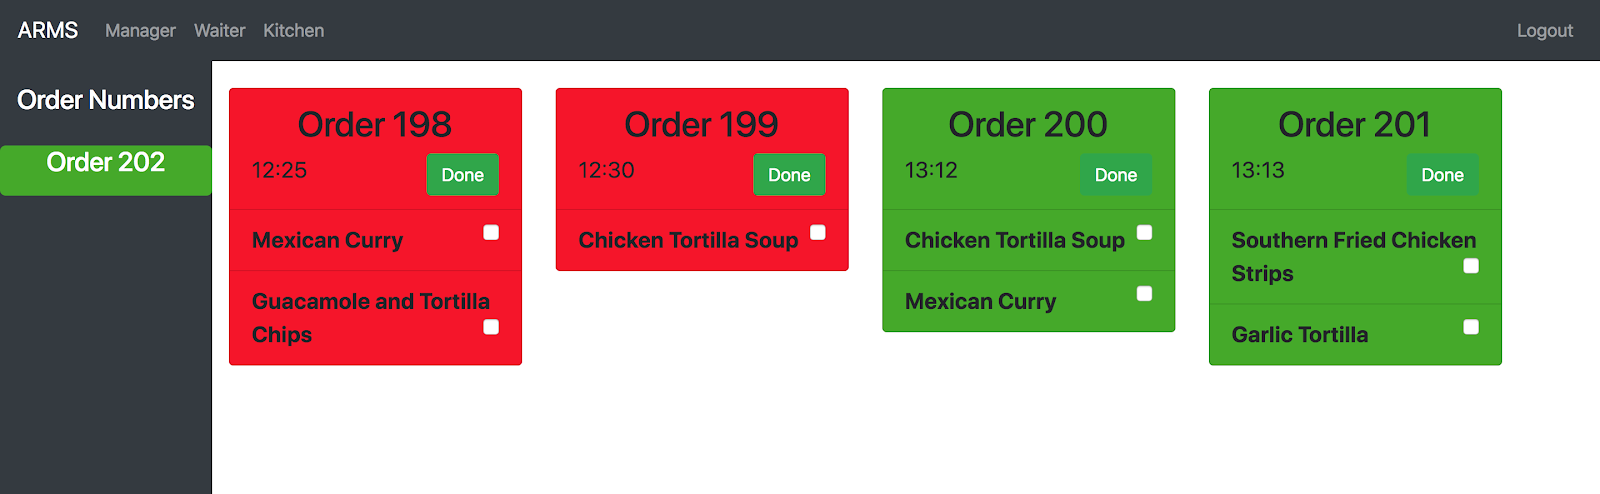
\includegraphics[width=10cm]{Kitchen1.png}
  \caption{The Kitchen Page}
  \label{fig:kitchen1}
\end{figure}

When orders are confirmed by the waiter a notification is shown for the kitchen, this also updates the page.

See \textit{Figure \ref{fig:kitchen2}}

\begin{figure}[H]
  \centering
  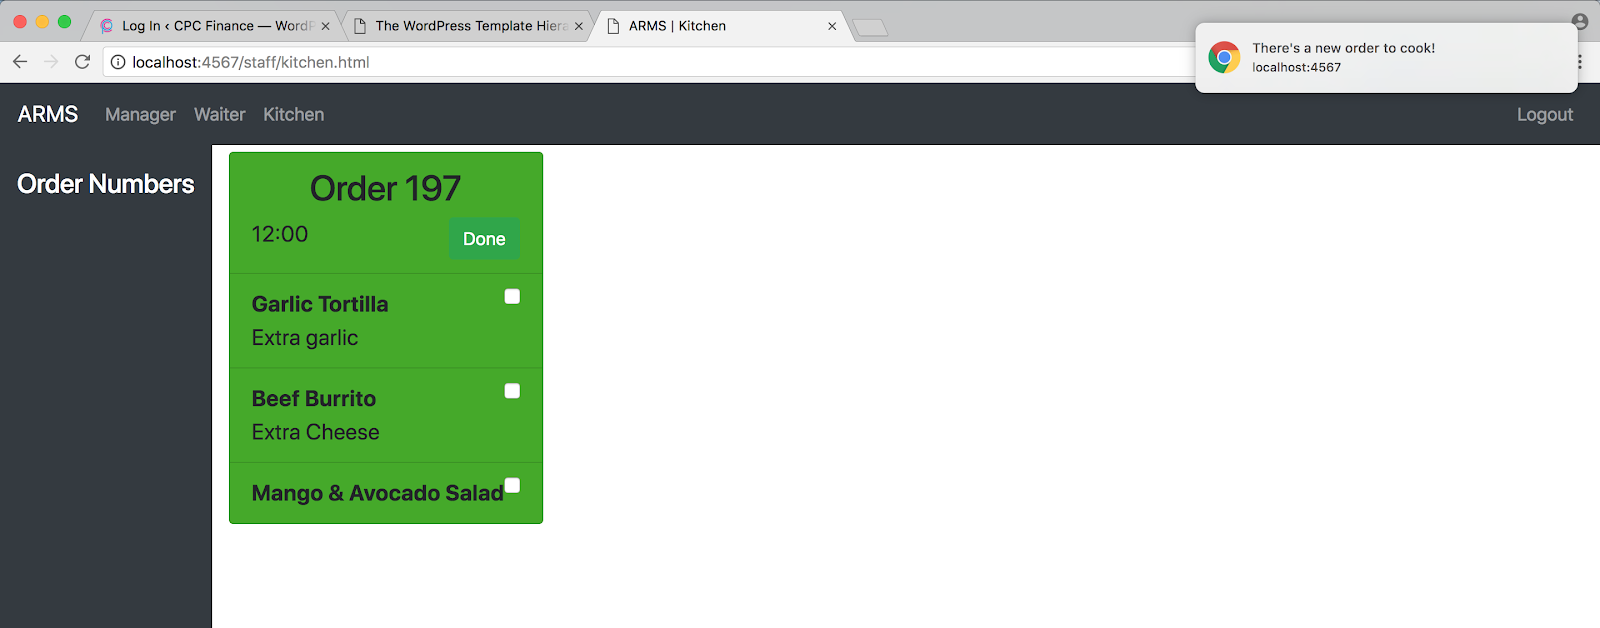
\includegraphics[width=10cm]{Kitchen2.png}
  \caption{Kitchen Notifications}
  \label{fig:kitchen2}
\end{figure}

\subsection*{Manager}
\subsubsection*{Manager Home Page}
This is the manager home page, see \textit{Figure \ref{fig:manMenu}}. You are taken here after logging in with a manager account. From here you can access the all of the manager pages and also the staff portals.

\begin{figure}[H]
  \centering
  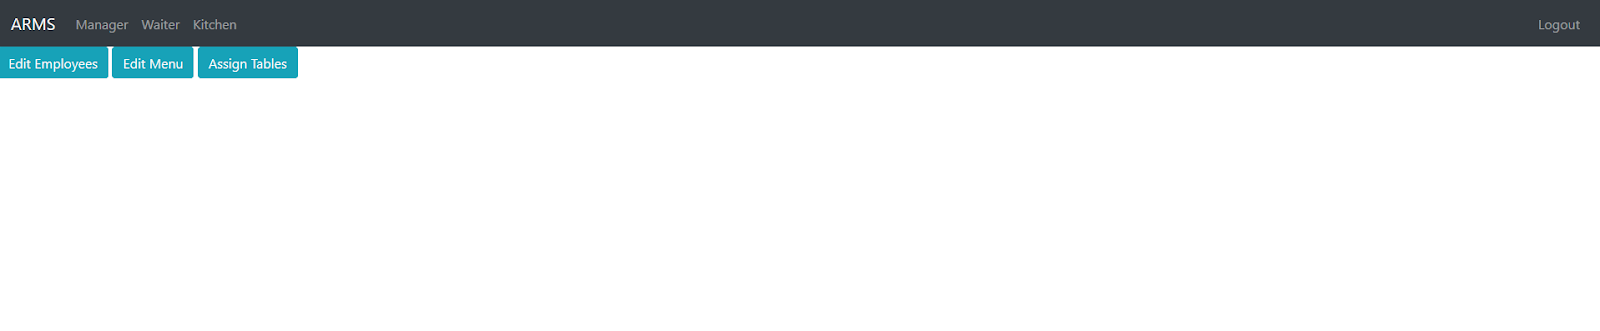
\includegraphics[width=10cm]{ManagerMenu.png}
  \caption{The Manager's Menu}
  \label{fig:manMenu}
\end{figure}

\subsubsection*{Edit Menu Page}
This page lists all the menu items currently on the franchises menu.
You can edit any item by clicking the yellow edit button next to it, or remove it from the menu by clicking the red cross.
Clicking the Show All Menu Items will also show the items which are not on the menu.

See \textit{Figure \ref{fig:editMenu1}}

\begin{figure}[H]
  \centering
  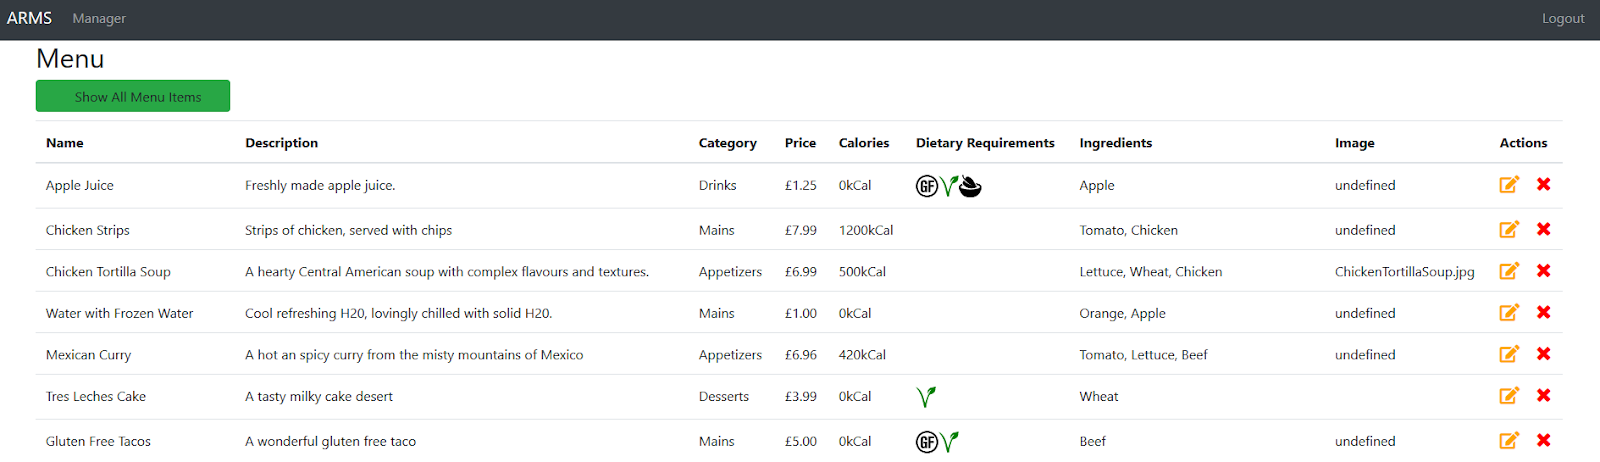
\includegraphics[width=10cm]{editMenu1.png}
  \caption{Editing Menu}
  \label{fig:editMenu1}
\end{figure}

If the item is not on the menu, it will have a green plus instead of a red cross. Clicking on that will add it to the franchise menu. If you want to add a new menu item which does not exist, you can select the Add New Menu Item button at the bottom of the page.

See \textit{Figure \ref{fig:editMenu2}}
\begin{figure}[H]
  \centering
  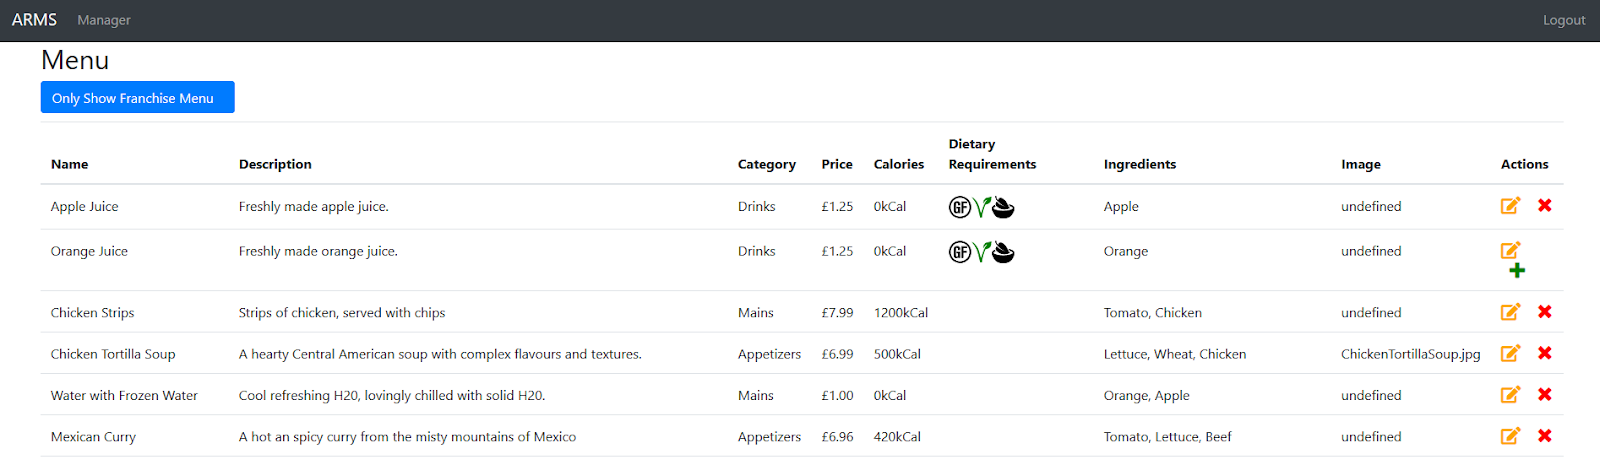
\includegraphics[width=10cm]{editMenu2.png}
  \caption{Editing Menu}
  \label{fig:editMenu2}
\end{figure}

Clicking this button will bring up a wizard which will guide you through the process of creating a new menu item.

See \textit{Figures \ref{fig:editWizard1}, \ref{fig:editWizard2} and \ref{fig:editWizard3}}

\begin{figure}[H]
  \centering
  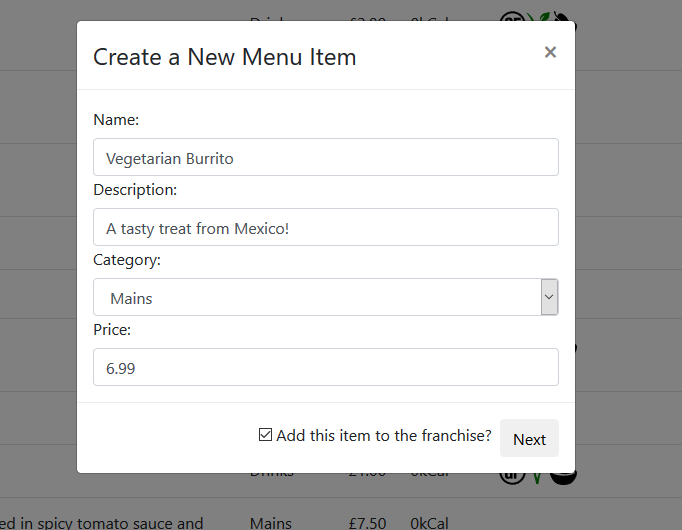
\includegraphics[width=5cm]{editWizard1.png}
  \caption{Editing Menu Wizard}
  \label{fig:editWizard1}
\end{figure}

\begin{figure}[H]
  \centering
  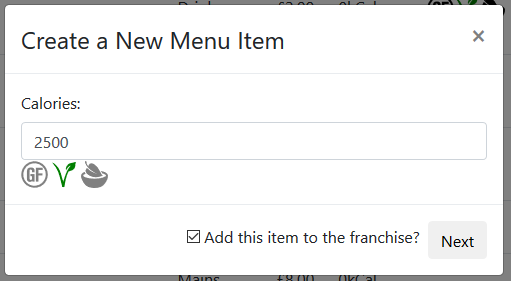
\includegraphics[width=5cm]{editWizard2.png}
  \caption{Editing Menu Wizard}
  \label{fig:editWizard2}
\end{figure}

\begin{figure}[H]
  \centering
  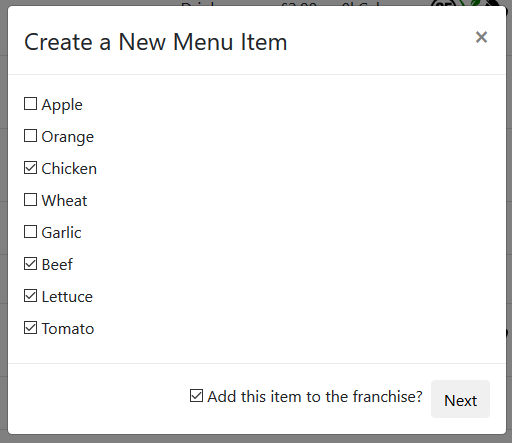
\includegraphics[width=5cm]{editWizard3.png}
  \caption{Editing Menu Wizard}
  \label{fig:editWizard3}
\end{figure}

\subsubsection*{Assign Tables Page}
This page loads all the waiters and the tables the are currently assigned to on the left hand side. On the right hand side is the list of all unassigned table.
The manager can unassign and assign tables using the arrow buttons.

See \textit{Figure \ref{fig:assign}}

\begin{figure}[H]
  \centering
  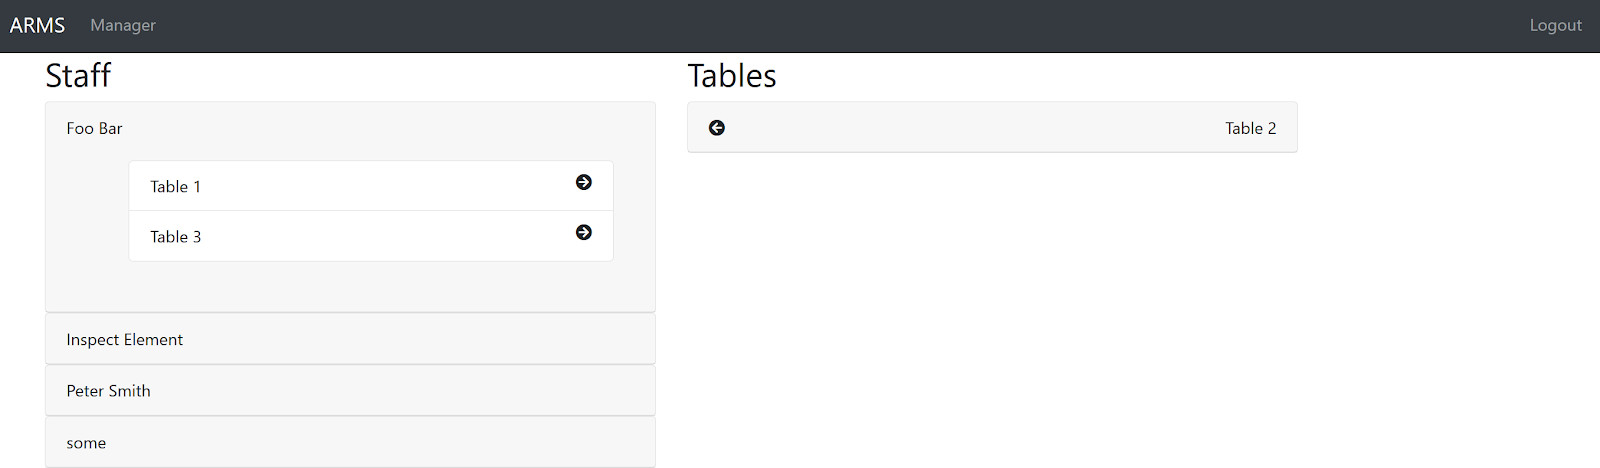
\includegraphics[width=5cm]{assignTables.png}
  \caption{Assign Tables Page}
  \label{fig:assign}
\end{figure}

\subsubsection*{Employee Page}
This page is used to create new staff, manage staff details and delete staff. You can click the Add Staff button to open the new staff form. Upon adding a staff member you will be prompted to enter a password for the user.

See \textit{Figure \ref{fig:employee1}}

\begin{figure}[H]
  \centering
  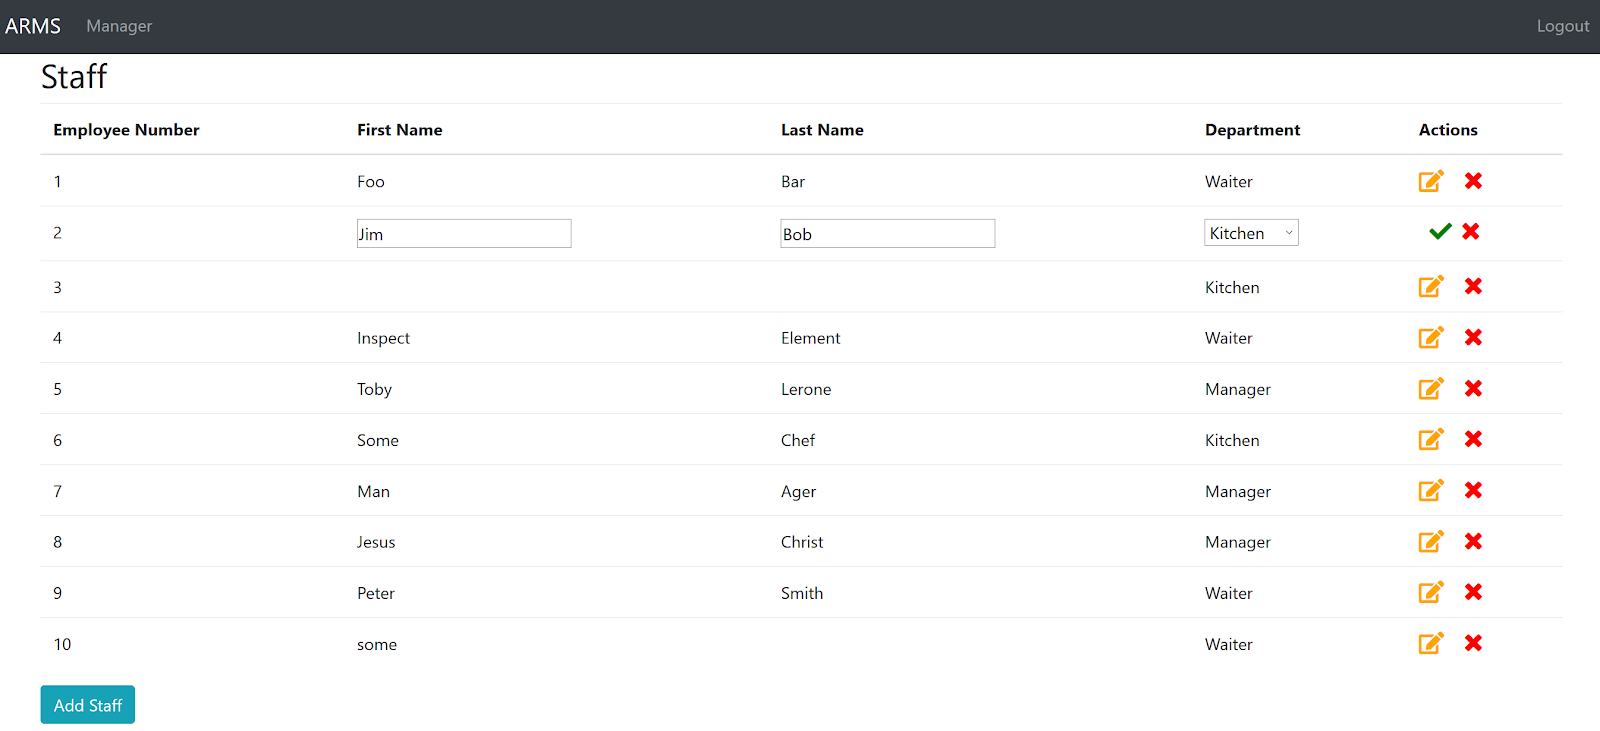
\includegraphics[width=5cm]{employee1.png}
  \caption{Edit Employee Page}
  \label{fig:employee1}
\end{figure}

Selecting the edit button will open the edit form for the selected user, where you can change the name and the department of the employee. You can click the green tick to send the changes. You can click the red cross to delete the employee.

See \textit{Figure \ref{fig:employee2}}
\begin{figure}[H]
  \centering
  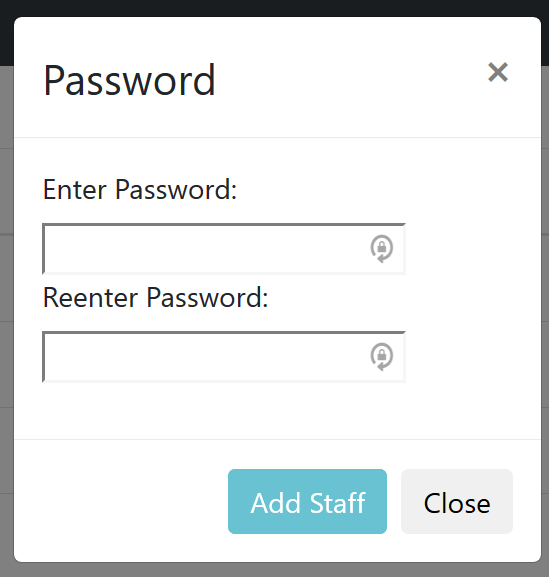
\includegraphics[width=5cm]{employee2.png}
  \caption{Edit Employee Page - Create Password}
  \label{fig:employee2}
\end{figure}

\section*{Server}
The server is responsible for providing communication and authentication between the user interface and the database.
We use Spark to handle the communication between the front end and the server itself. We have created numerous classes for the purpose, more detail is provided in \textit{\nameref{sec:endpoints}}.

Also handled by the server is the communication and the creation of the database, we use the Hibernate ORM and JPA to create and communicate to the PostgreSQL database. More detail on how this is done is provided in \textit{\nameref{sec:database}}.

\section*{Database}

We have a database with 19 related tables, see \textit{Figure \ref{fig:data}} 

The database stores everything including the staff, the menu and the customers orders. 
It also stores the logged in sessions and the data needed for push notifications.
The database was designed to allow the user to start multiple orders and store them onto a transaction that allows the users to pay for all there orders in one go.

\begin{figure}[H]
  \centering
  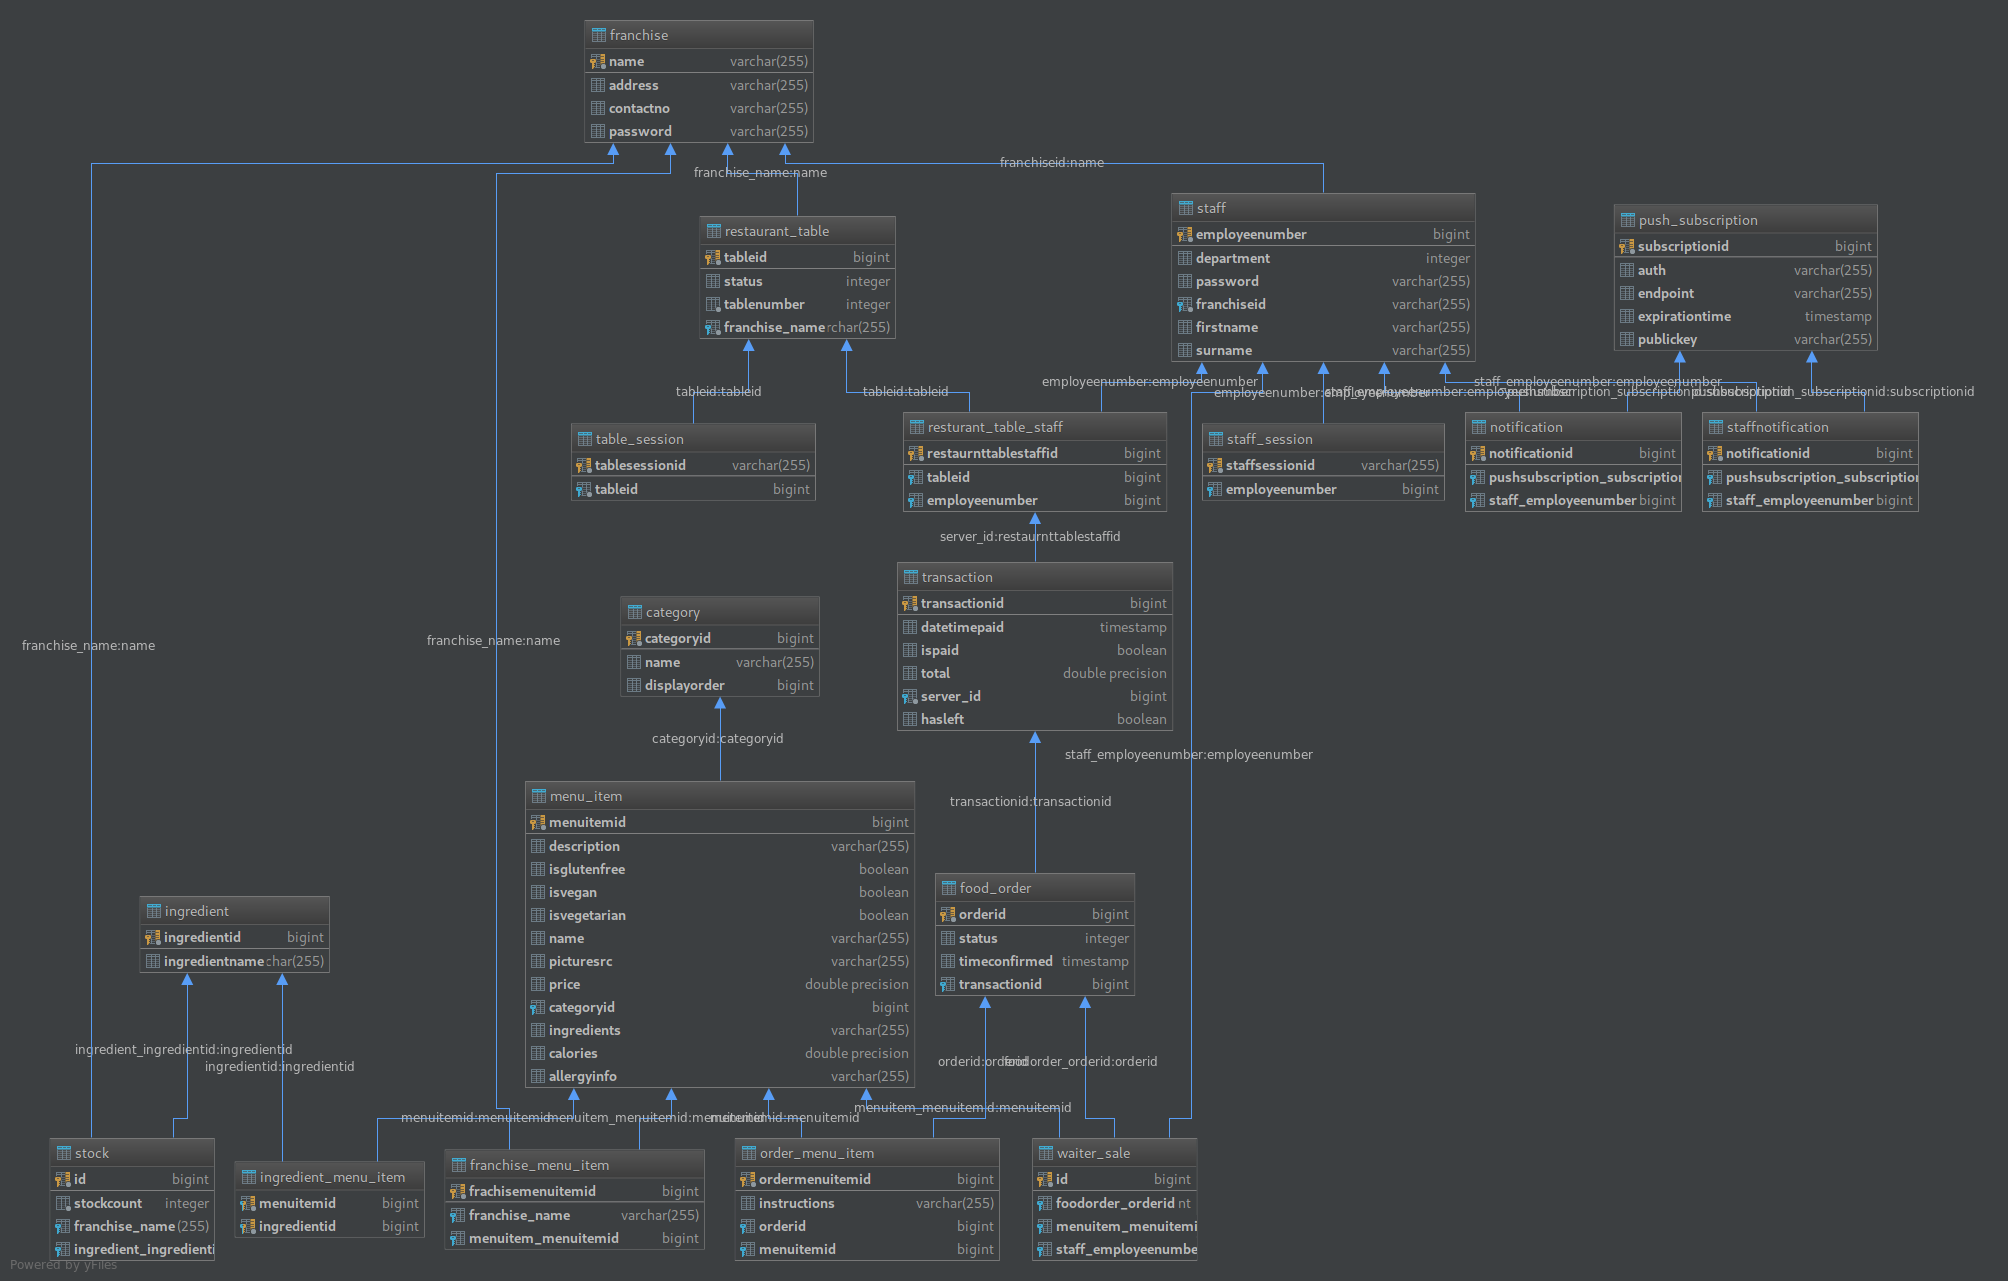
\includegraphics[width=15cm]{database.png}
  \caption{Generated by DataGrip}
  \label{fig:data}
\end{figure}

\chapter*{Description Of Packages}
\section*{Database}\label{sec:database}
\subsection*{Implemented Components}
This package implements the following components:
\begin{itemize}
  \item A fully relational database in hopefully third normal form. All created with Hibernate ORM.

    See \textit{\href{run:../JavaDoc/database/tables/package-summary.html}{Table Overview}} for more details.
  \item A Database Manager Singleton for easy access to creating JPA Entity Managers, without the need of creating more than one factory.

    See \textit{\href{run:../JavaDoc/database/package-summary.html}{Database Overview}} for more details.
\end{itemize}

\section*{Endpoints}\label{sec:endpoints}
\subsection*{Implemented Components}
This package contains classes that link the front end to the database.
\begin{itemize}
  \item Authentication classes to authenticate a users login to stop unauthorized access. 

    See \textit{\href{run:../JavaDoc/endpoints/authentication/package-summary.html}{Authentication Overview}} for details.
  \item Ingredient classes to provide end points that interact with the ingredient table in the database.

    See \textit{\href{run:../JavaDoc/endpoints/ingredient/package-summary.html}{Ingredients Overview}} for details.
  \item Manger classes to provide the end points necessary to create the implemented manager user stories.

    See \textit{\href{run:../JavaDoc/endpoints/manager/package-summary.html}{Manger Overview}} for details.
  \item Menu classes to provide the end points needed to load and edit the menu.

    See \textit{\href{run:../JavaDoc/endpoints/menu/package-summary.html}{Menu Overview}} for details.
  \item Notification classes that provide our push notification service, including auto updating the web pages.

    See \textit{\href{run:../JavaDoc/endpoints/notification/package-summary.html}{Notification Overview}} for details.
  \item Order classes to provide the ability to create, view and edits for both the customer view and the waiter view.

    See \textit{\href{run:../JavaDoc/endpoints/order/package-summary.html}{Order Overview}} for details.
  \item Payment classes to provide the Stripe functionality so they customers can pay by card.

    See \textit{\href{run:../JavaDoc/endpoints/payment/package-summary.html}{Payment Overview}} for details.
  \item Table classes to get the list of table, change there status and change which waiters are assigned to which table.

    See \textit{\href{run:../JavaDoc/endpoints/tables/package-summary.html}{Tables Overview}} for details.
  \item Transaction classes to allow the front end to get details on the current transaction.

    See \textit{\href{run:../JavaDoc/endpoints/transaction/package-summary.html}{Transaction Overview}} for details
\end{itemize}

\section*{Static}\label{sec:static}
\subsection*{Implemented Components}
\begin{itemize}
  \item An AJAX Wrapper to easily make Post and Get requests.

    See \textit{\href{run:../JSDoc/module-AJAX_Wrapper.html}{AJAX Wrapper}} for more details.
  \item A Customer landing page, that allows the users to start an order.

    See \textit{\href{run:../JSDoc/module-Customer-Home.html}{Customer Home}} for more details.
  \item A Customer menu page, that allows the customer to view the menu and add items to there order.

  See \textit{\href{run:../JSDoc/module-Customer-Menu.html}{Customer Menu}} for more details.
  \item A Waiter page, that allows a waiter to see the current orders for a table, confirm and edit those orders. As well as manage the status of tables.

    See \textit{\href{run:../JSDoc/module-Waiter.html}{Waiter}} for more details.
  \item A Kitchen page, that allows kitchen staff the orders that need to be cooked and indicate when they are done cooking.

    See \textit{\href{run:../JSDoc/module-Kitchen.html}{Kitchen}} for more details.
  \item An Edit Menu page for the manager, so the manager can update the menu.

    See \textit{\href{run:../JSDoc/module-Manager-Menu.html}{Edit Menu}} for more details.
  \item An Edit Employee page for the manager, so the manager can edit and create new employees.

    See \textit{\href{run:../JSDoc/module-Manager-Employee.html}{Edit Employee}} for more details.
  \item An Assign Tables page for the manager, that allows them to assign waiters to table.

    See \textit{\href{run:../JSDoc/module-Manager-Assign-Tables.html}{Assign Tables}} for more details.
  \item Push notifications that allow both waiters and kitchen staff to be kept up to date.
    
    See \textit{\href{run:../JSDoc/module-Register-Service-Worker.html}{Notifications}} for more details.
\end{itemize}

\section*{Utility}\label{sec:util}
\subsection*{Implemented Components}
This package implements a GSON Singleton to limit the need of creating numerous GSON objects for each of the end point classes.

See \textit{\href{run:../JavaDoc/util/package-summary.html}{Utility Package}} for more details.

\chapter*{User Stories}
\section*{Fully Completed}
These are the completed user stories.
\subsection*{Customer Stories}
\begin{itemize}
  \item Electronic Payment
  \item View Menu
  \item Ordering
  \item Menu Filtering
  \item Calling The Waiter
  \item Allergies And Calories
  \item Food Pictures
  \item Order Tracking
  \item Intuitive Ordering
\end{itemize}

\subsection*{Waiter Stories}
\begin{itemize}
  \item Notification For Delivery
  \item Cancel Order
  \item Order Times
  \item Payment Information
  \item Order Confirmation
  \item Table Assignment
  \item Mark Order as Delivered
  \item Client Needs Help
  \item Add Extra Sales
  \item Change Status Of An Order
\end{itemize}

\subsection*{Kitchen Stories}
\begin{itemize}
  \item Notify Waiters
  \item Confirmed Customer Order
  \item Order Times
\end{itemize}

\subsection*{Manager Stories}
\begin{itemize}
  \item Assign Tables
  \item Set Prices
\end{itemize}

\section*{Nearly Completed}
These stores are worthy of a mention as they are very nearly finished.

\subsection*{Manager Stories}
\begin{itemize}
  \item Adjust Menu:
    The only feature left uncompleted is uploading an image to the new menu item or when editing a menu item.
  \item Add Staff:
    The only feature left is the ability to reset a users password.
\end{itemize}

\chapter*{Statement of Relative Contribution}
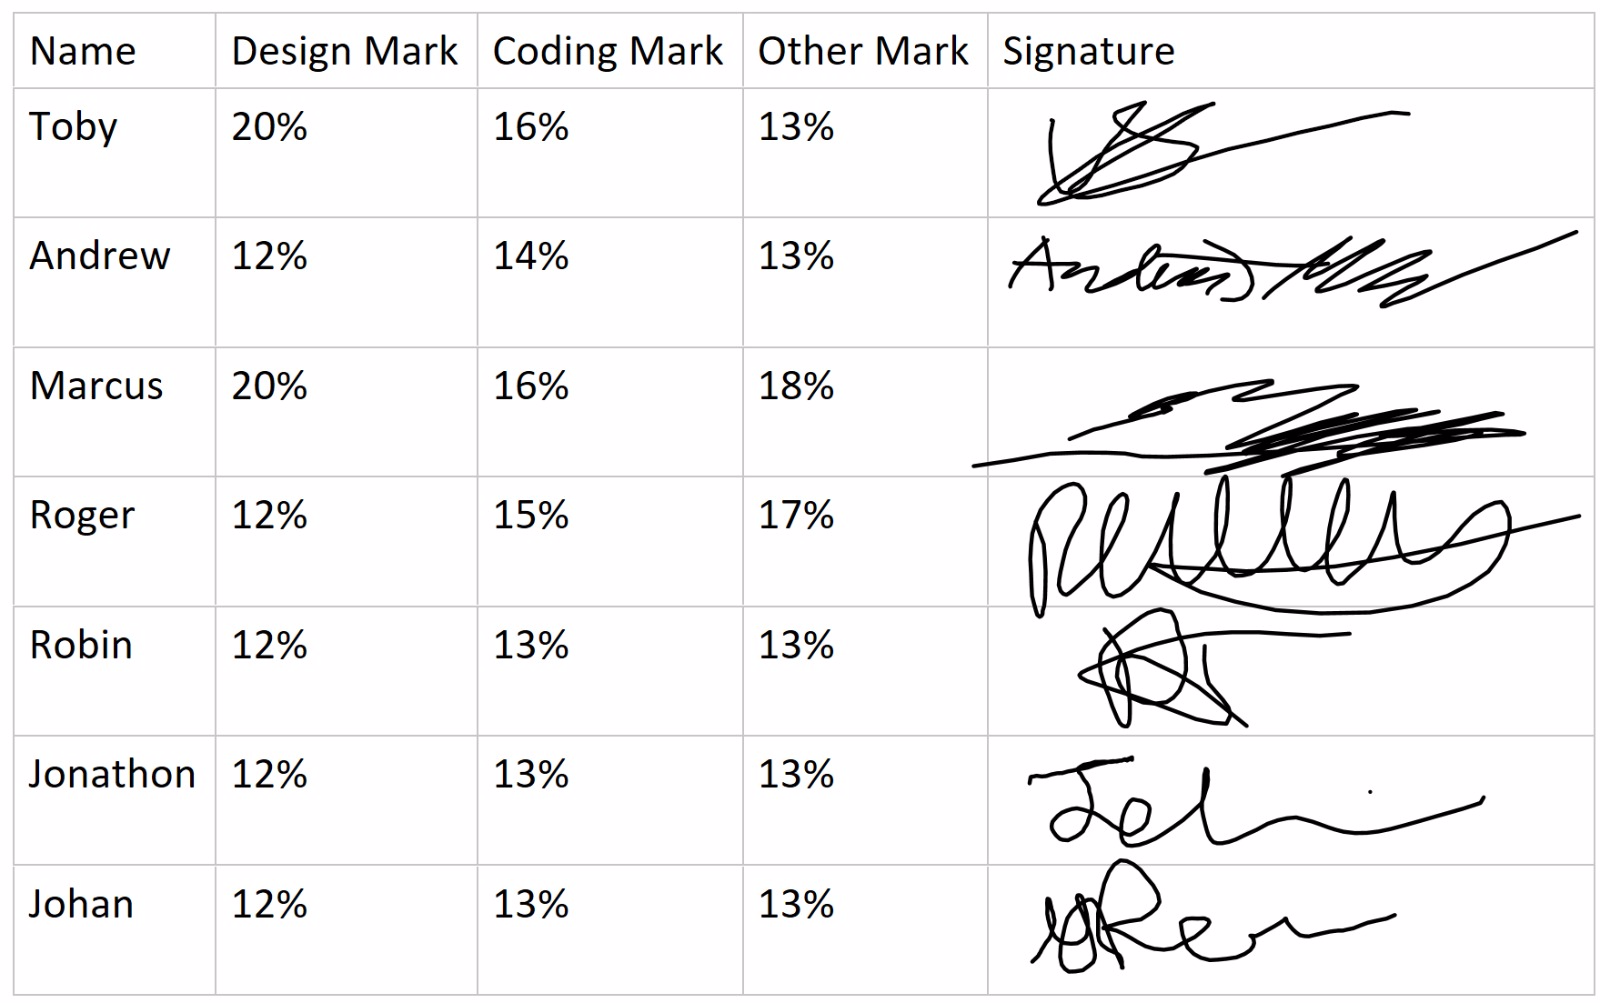
\includegraphics[width=15cm]{StateOfCont.png}

\end{document}
